\section{АНАЛИЗ СУЩЕСТВУЮЩИХ РЕШЕНИЙ}
\label{sec:solution}

\subsection{EasyScan}
EasyScan - это простой инструмент для сканирования документов и изображений, который позволяет пользователям выполнять сканирование на нескольких типах платформ принтера. EasyScan использует стандартные возможности Twain, позволяющие всем пользователям Windows загружать, устанавливать и использовать это приложение. 

\begin{figure}[h!]
	\centering
	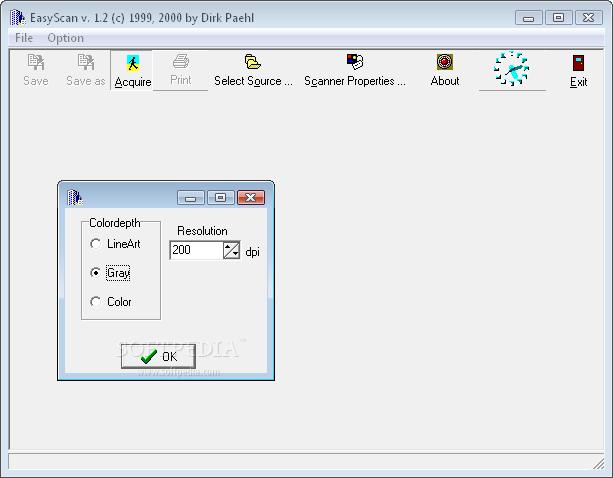
\includegraphics[scale=0.48]{easyscan.png}
	\caption{EasyScan}
\end{figure}

Преимущества:
\begin{itemize}
	\item использование Twain в программе EasyScan делает его отличным от других приложений, поскольку его можно использовать на нескольких платформах;
	\item программа позволяет сканировать с различной глубиной цвета, включая 256, 16 и более т.д; 
	\item возможность поворачивать изображение или выбирать определенный RGB канал; 
	\item простота установки. EasyScan работает на большинстве операционных систем Windows и может быть использован в течение нескольких минут после завершения процесса загрузки; 
	\item после открытия приложения у вас есть возможность изменить многие параметры сканирования, включая разрешение, размер, ориентацию, цвет, увеличить или уменьшить масштаб изображения и т.д;
\end{itemize}

Недостатки:
\begin{itemize}
	\item EasyScan не обновлялся с 2011 года;
	\item для пользователей, не знакомых с компьютерами настройка программы может оказаться сложной;
\end{itemize}

\subsection{NAPS2} 
NAPS2 легко сканирует с любыми выбранными настройками. Также можно настроить несколько профилей для различных устройств и конфигураций. После завершения сканирования получившийся документ можно сохранить файл в PDF, TIFF, JPEG, PNG и т.д., отправить по электронной почте или распечатать. Для этого понадобится сделать всего лишь пару кликов мышью.


\begin{figure}[h!]
	\centering
	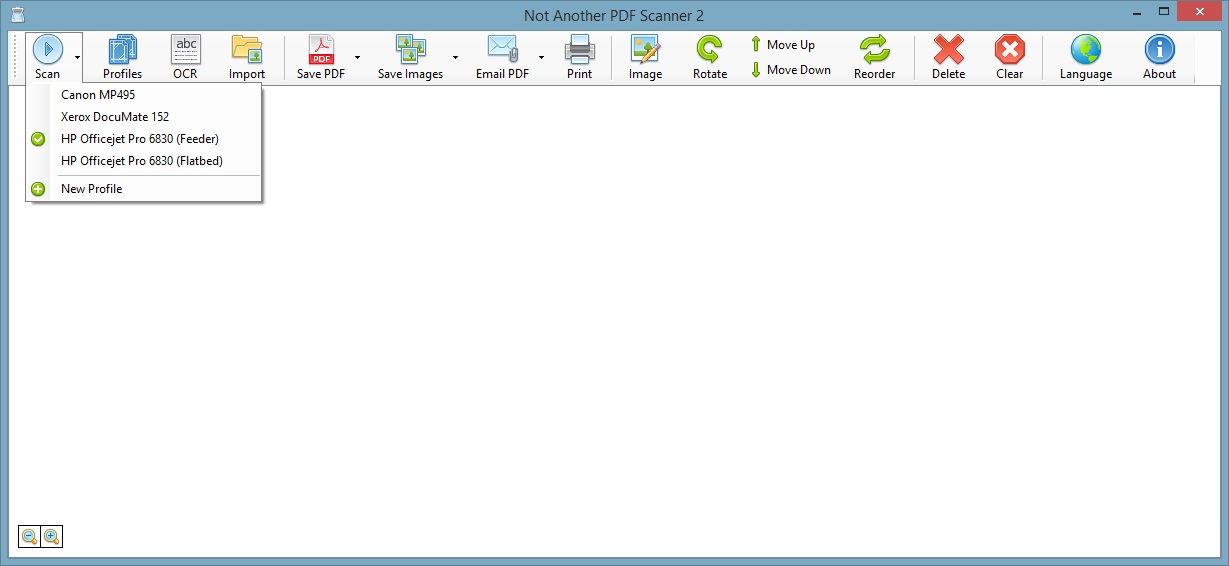
\includegraphics[scale=0.5]{naps2.jpg}
	\caption{NAPS2}
\end{figure}

Возможности:
\begin{itemize}
	\item совместимость с WIA и TWAIN;
	\item функция вращения, обрезки и упорядочивания отсканированных изображений;
	\item распознавание текста с помощью OCR;
	\item дополнительный интерфейс командной строки (CLI) для автоматизации и скриптов;
	\item MSI установщик и конфигурация на уровне приложений, доступная для развертывания групповой политики (GPO);
	\item доступны портативные архивы (не требует установки);
\end{itemize}

\subsection{PaperScan}
Программа имеет малый вес и не требовательна к ресурсам компьютера, поэтому ее очень удобно использовать, если при сканировании вам понадобилось изменить документ или изображение в нем.

Программу можна использовать как дополнение к пакету офисных программ.

\begin{figure}[h!]
	\centering
	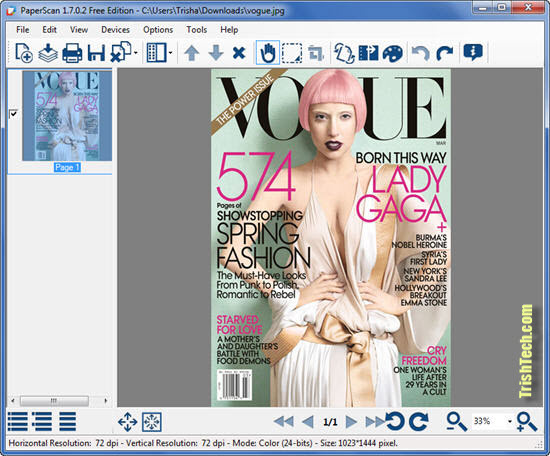
\includegraphics[scale=0.78]{paperscan.jpg}
	\caption{PaperScan}
\end{figure}

Возможности:
\begin{itemize}
	\item работа с любым типом графических файлов;
	\item поддержка любого сканера;
	\item стирание границ и следов пробивки;
	\item черно-белый режим для цветных фотографий и картинок;
	\item работа с изображением: редактирование яркости, контраста, гаммы и других основных характеристик;
	\item галерея эффектов и фильтров для изображений;
\end{itemize}

\subsection{WinScan2PDF}
WinScan2PDF – это очень маленькая и удобная программа, которая дает возможность в значительной мере упростить процесс сканирования различных документов с их дальнейшим сохранением на жестком диске компьютера, в формате PDF.

Программа не нуждается в виртуальном принтере и не требует инсталляции дополнительных программ. Для выполнения задачи нужно только запустить WinScan2PDF и в окне приложения выбрать источник, после кликнуть по соответствующей кнопке – и все готово! После таких простых действий нужно только сохранить полученный документ в формате PDF.

\begin{figure}[h!]
	\centering
	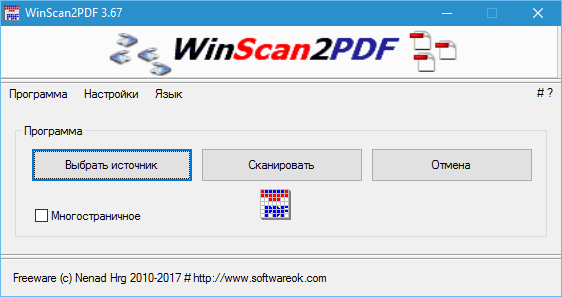
\includegraphics[scale=0.78]{winscan2pdf.png}
	\caption{WinScan2PDF}
\end{figure}

Функциональные возможности:
\begin{itemize}
	\item быстрое сканирование документов в любом количестве с дальнейшим сохранением в формате PDF;
	\item возможность работы прямо с USB-накопителя, без необходимости установки на жесткий диск компьютера;
	\item небольшой размер и минимальные требования к системным ресурсам;
	\item "Быстрый" и удобный интерфейс WinScan2PDF, поддержка русского языка;
\end{itemize}